
%%%%%%%%%%%%%%%%%%%%%%%%%%%%%%%%%%%%%%%%
%%%%%%%%%%%  Note Template   %%%%%%%%%%%
%%%%%%%%%%%     20170717     %%%%%%%%%%%
%%%%%%%%%%% Jeffrey M. Moore %%%%%%%%%%%
%%%%%%%%%%%%%%%%%%%%%%%%%%%%%%%%%%%%%%%%

%%%%%%%%%%%%%%%%%%%%%%%%%%%%%%%%%%%%%%%%
%%%%%% APS/PRL formatted document %%%%%%
%%%%%%%%%%%%%%%%%%%%%%%%%%%%%%%%%%%%%%%%
%\documentclass[aps,prl,twocolumn,groupedaddress]{revtex4}
%\documentclass[aps,prl,twocolumn,showpacs,superscriptaddress,groupedaddress]{revtex4}  % for review and submission
%\setcitestyle{super} % for superscripted citations
%%%%%%%%%%%%%%%%%%%%%%%%%%%%%%%%%%%%%%%%

%%%%%%%%%%%%%%%%%%%%%%%%%%%%%%%%%%%%%%%%
%%%%%%%% Article document class %%%%%%%%
%%%%%%%%%%%%%%%%%%%%%%%%%%%%%%%%%%%%%%%%
\documentclass[11pt]{article}
\usepackage[width=7.0in, height=9.0in, head=0.0in, foot=0.5in, headsep=0.0in]{geometry} 
\usepackage{setspace}  % useful in changing vertical spacing temporarily.
\usepackage{authblk}   % for affiliations 
%\usepackage[superscript, biblabel]{cite} % for superscripted citations 
%%%%%%%%%%%%%%%%%%%%%%%%%%%%%%%%%%%%%%%%

\usepackage{graphicx}  % needed for figures
\usepackage{dcolumn}   % needed for some tables
\usepackage{bm}        % for math 
\usepackage{amssymb}   % for math 
\usepackage{amsmath}   % for math
\usepackage{mathtools} % for math
\usepackage{tabularx}  % for tables
\usepackage{lipsum}    % used for filler text
%\usepackage{caption}
\usepackage{subcaption}
\usepackage[ruled,vlined]{algorithm2e}

\graphicspath{{figs/}} % specify figure folder
%\linespread{1.3}       % change line spacing

%%% for correct hyphenation %%%
\hyphenation{ALPGEN} \hyphenation{EVTGEN} \hyphenation{PYTHIA}

%%% For alpha-labeled sections %%%
%\renewcommand{\thesection}{\Alph{section}}
\begin{document}

\captionsetup{font=normalsize,labelfont={bf,sf}}
\captionsetup[sub]{font=small,labelfont={bf,sf}}

%%% For horizontal space %%%
\newcommand{\inden}[1]{\mbox{} \hspace{#1} } 

\title{\bf{Statistical Modeling Final Project}} 
\author{Jeffrey M. Moore} 

%%% Standard affiliation %%%
%\affil{Department of Physics, University of Colorado, Boulder, Boulder, CO 80309}

%%% REVTEX4 affiliation %%%
%\affiliation{Department of Physics, University of Colorado, Boulder, Boulder, CO 80309}

\date{\today}

%%% REVTEX4 abstract before maketitle %%%
%\begin{abstract}
  %\lipsum[1]
%\end{abstract}

%\pacs{}
\maketitle

%%% Standard abstract after maketitle %%%
%\abstract{\lipsum[1]}

%%%%%%%%%%%%%%%%%%%%%%%%%%%%%%%%%%%%%%%%

%%% Sections are not used in PRL papers %%%
%%% When using sections in standard format: \section*{Unnumbered Section} %%%

 
\section{\label{sec:intro}Introduction}
Given two consecutive, random years of average monthly temperature data for fifty-one US cities, as well as the monthly electricity usage for those cities during those years, I will be constructing a statistical model to predict a third year of monthly electricity usage for Denver, Colorado given its average monthly temperature for that year. I will start by exploring the data in Section~\ref{sec:explore}, then I will discuss my model selection process in Section~\ref{sec:model}. I will then discuss the results and analyses of the model in Section~\ref{sec:results} and summarize my conclusions in Section~\ref{sec:conclusion}.
\section{\label{sec:explore}Exploratory Analysis}
In order to visualize the data, I plotted the temperature and electricity usage (from here on referred to as energy usage) as a function of time for both years (see Fig.~\ref{fig:exploratory1}). The approximate trend appears to be that temperatures are lowest in December/January and highest in July/August, and energy usage being lowest in July/August and highest in December/January. While the structure of the time-series data is similar between cities, the variance of temperature and energy usage differ greatly across the population.

Visualizing the direct temperature/energy relationship, I plotted the energy usage data as a function of temperature, while only differentiating data by the year the data was taken (see Fig.~\ref{fig:exploratory2}. While one year was quite a bit warmer than the other, there appears to be one underlying relationship between temperature and energy usage that remains static, which is good for a model that proposes to predict the energy usage for a third, random year.

\begin{figure}[ht] \centering
  \begin{subfigure}{0.49\textwidth}
    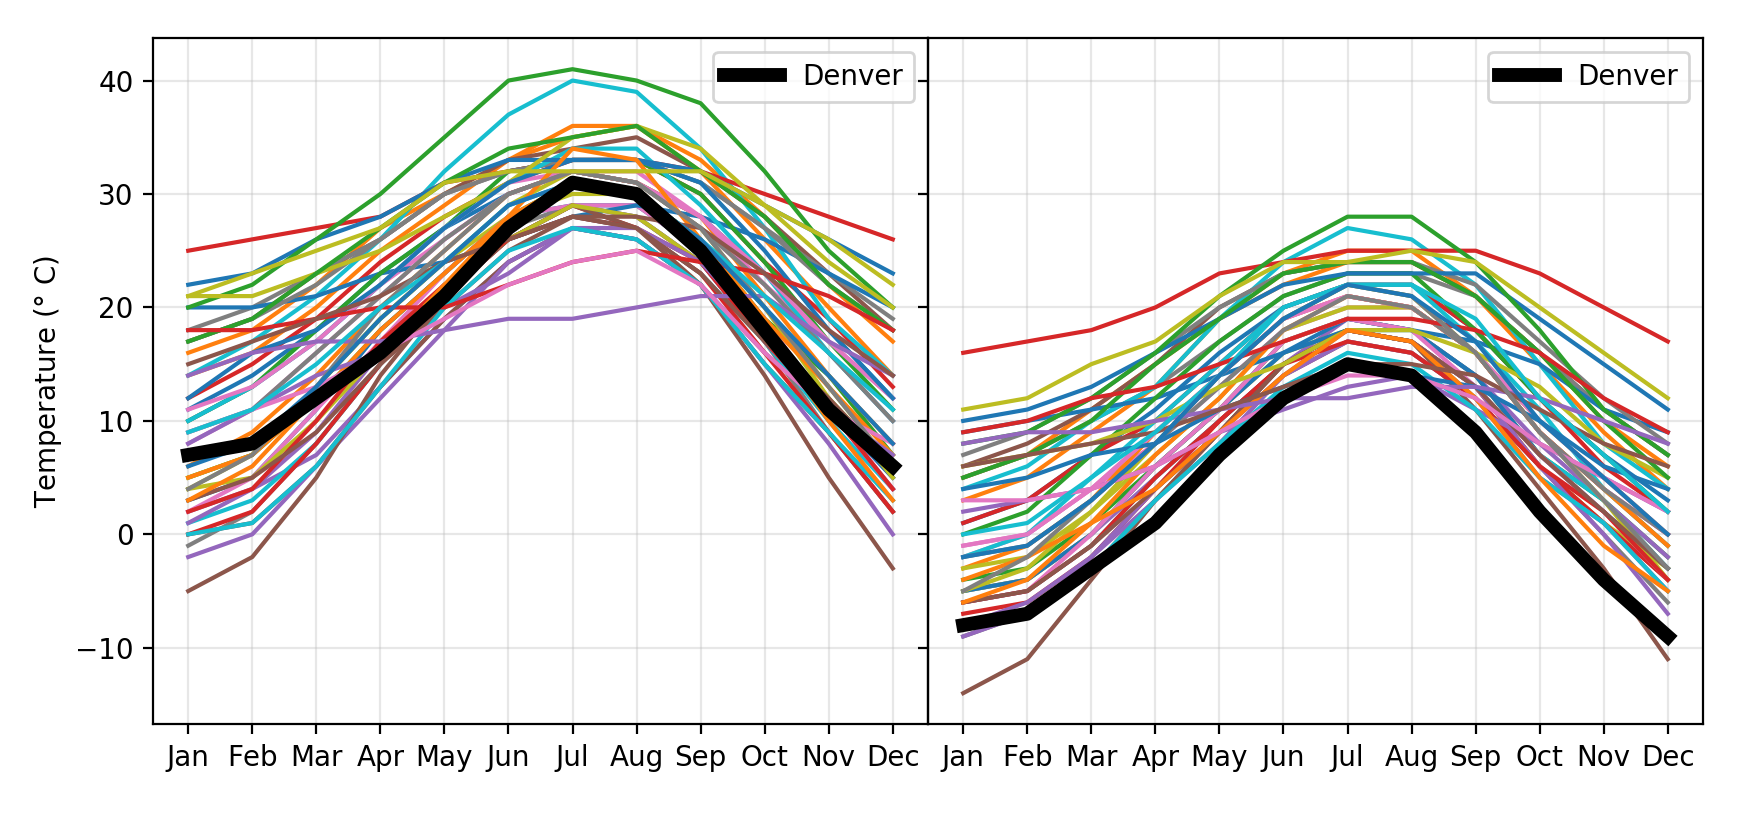
\includegraphics[width=\textwidth]{exploratory1b.png}
    \caption{Average monthly temperature (in $^\circ$Celsius) of cities over time for two random, non-consecutive years.}
    \label{fig:temp_time}
  \end{subfigure}%
  \hfill
  \begin{subfigure}{0.49\textwidth}
    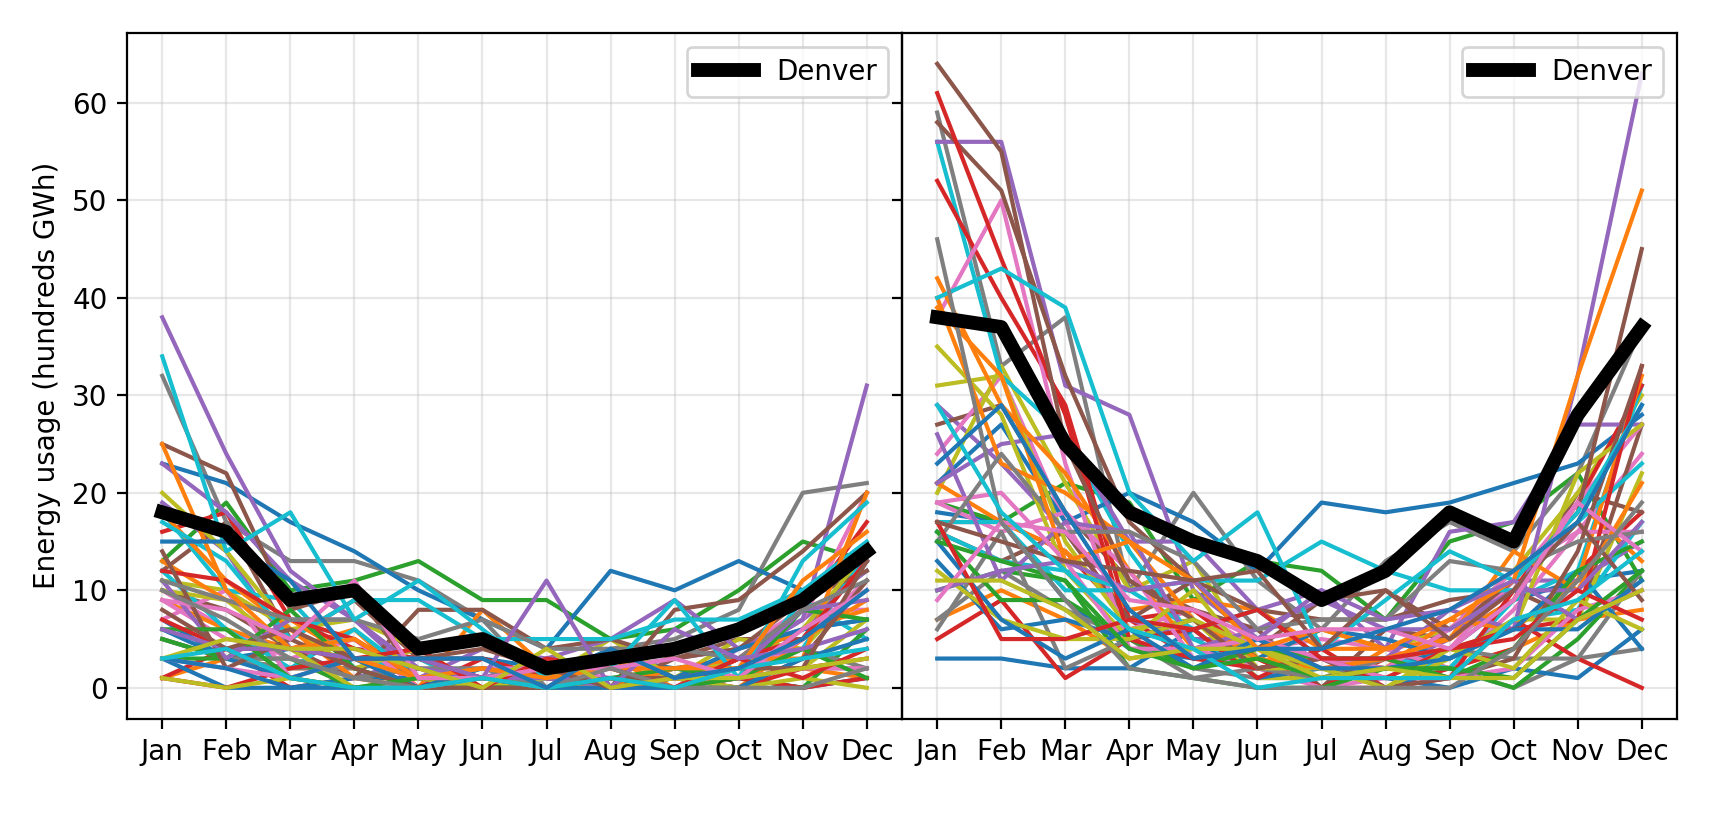
\includegraphics[width=\textwidth]{exploratory1a.png}
    \caption{Energy usage (in 100 GWh) of cities over time for two random, non-consecutive years.}
    \label{fig:energy_time}
  \end{subfigure}
  \caption{Plots depicting time-series data of all 51 US cities considered. The data of Denver, CO is darkened for qualitative comparison.}
  \label{fig:exploratory1}
\end{figure}

It is also clear given the structure of the data that the relationship between temperature and energy usage is non-linear, and exhibits what appears to be an exponential increase in energy usage as temperatures get lower. Assuming that the relationship is, in fact, exponential with respect to temperature, this suggests that a logarithmic transformation of the data by the function
\begin{equation} \label{eqn:g}
  g(y) = \ln(y+1)
\end{equation}
could be used to linearize the data. Plotting the relationship between $g(\text{energy usage})$ and temperature, the transformed data appears well suited for a linear model, especially when considering observations from the city of Denver independent of other cities, as I'll discuss further in the next section.

\begin{figure}[ht] \centering
  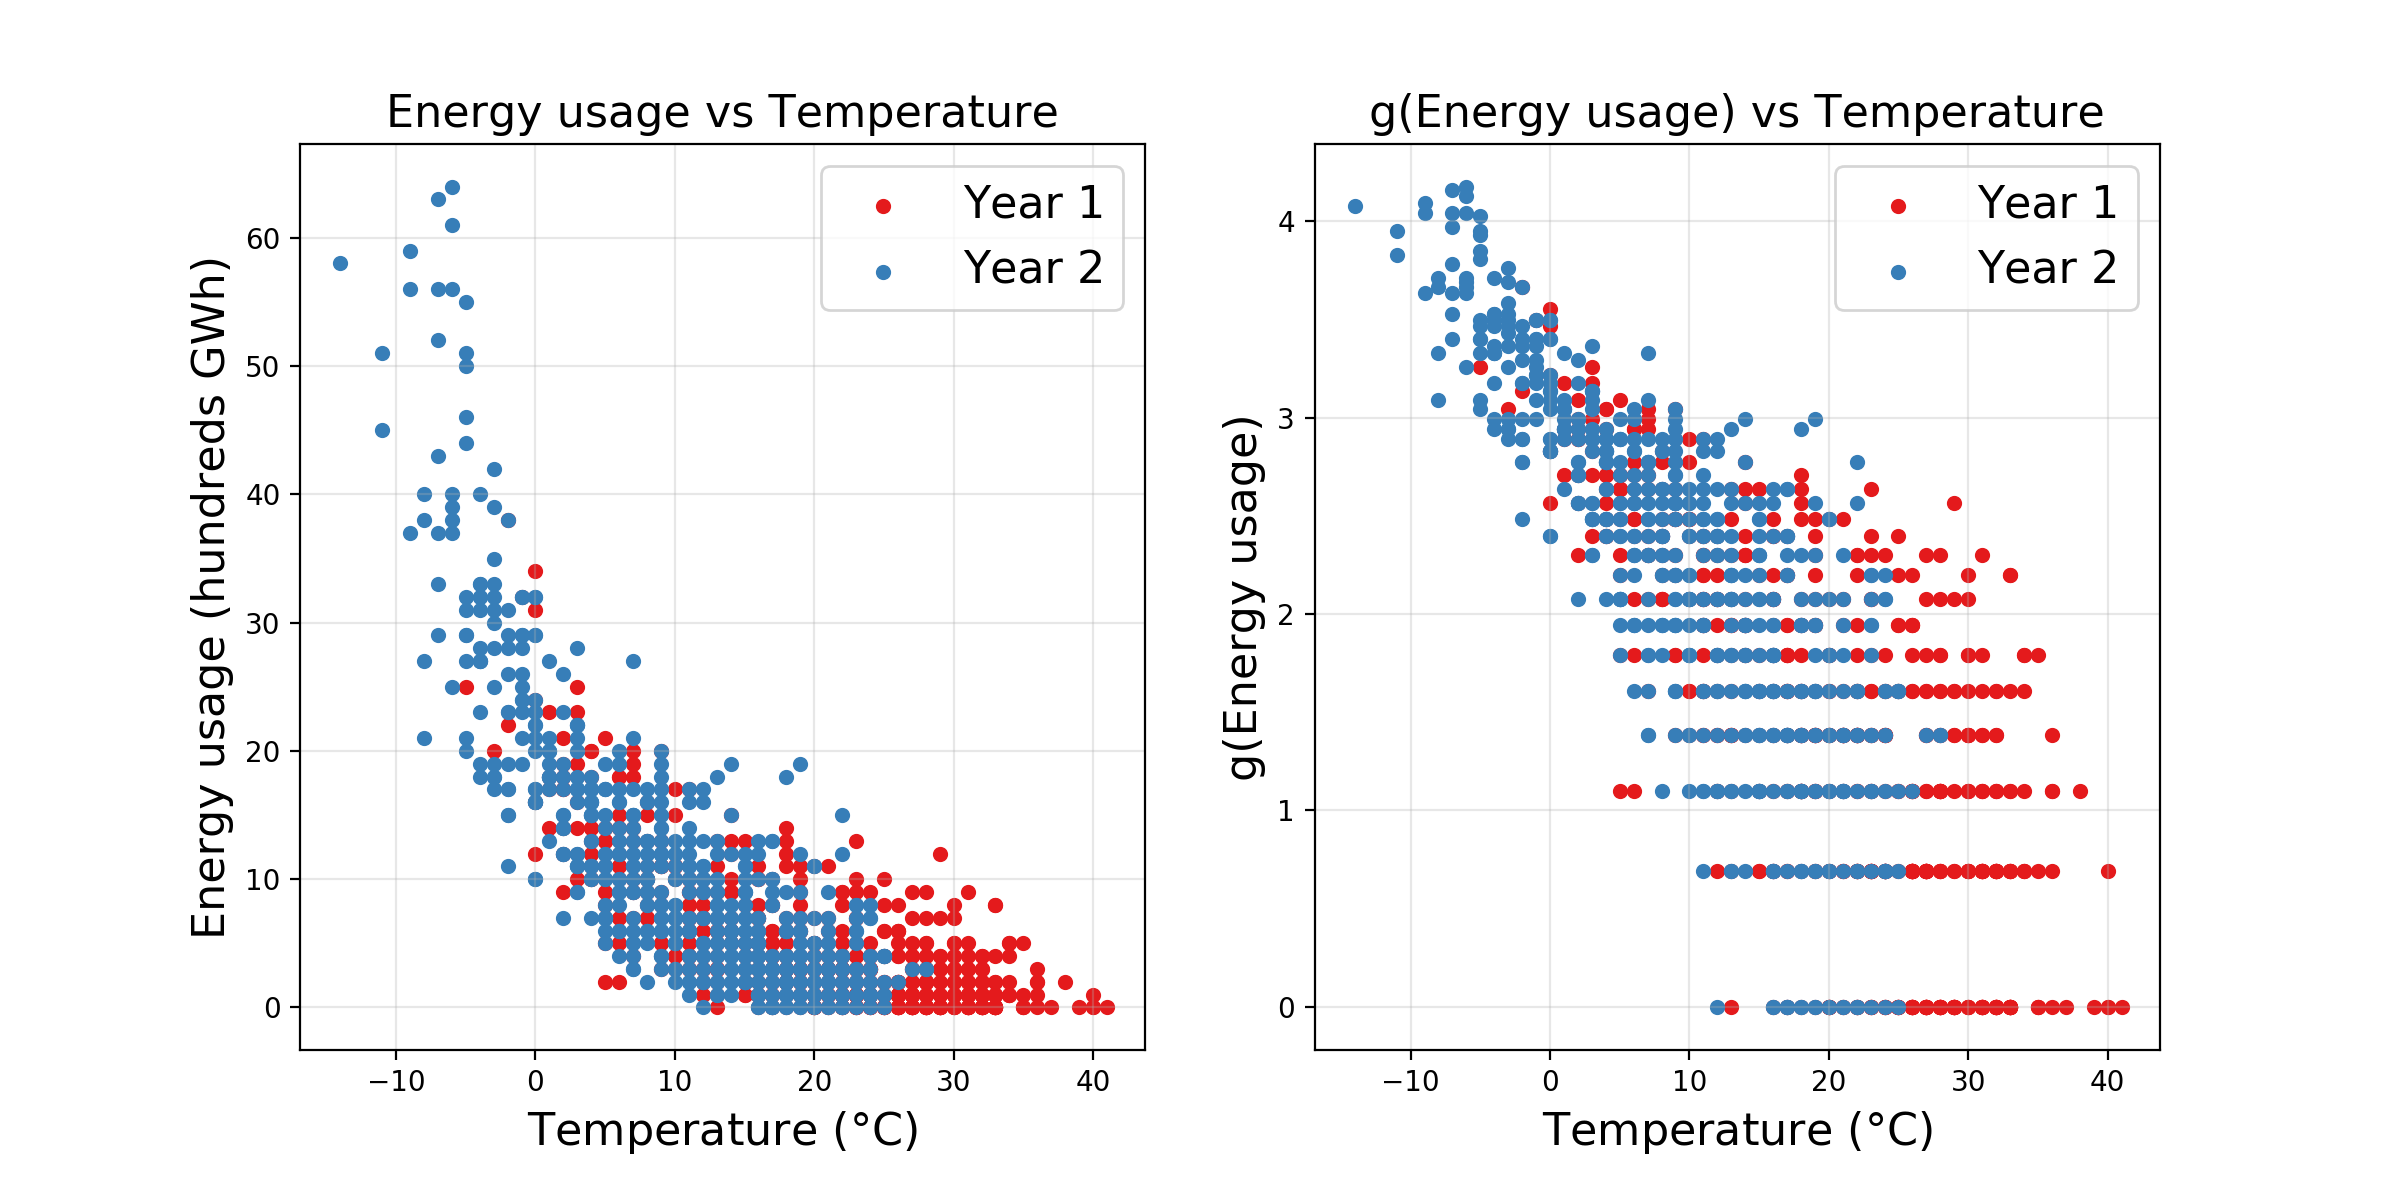
\includegraphics[width=0.9\textwidth]{exploratory2.png}
  \caption{Plots of the relationship between energy usage (in hundreds of GWh) vs temperature ($^\circ$Celcius) with observations segregated by year. The first plot visualizes the raw relationship, whereas the second explores the transformed (logarithmic) relationship.}
  \label{fig:exploratory2}
\end{figure}

\begin{figure}[ht] \centering
  \begin{subfigure}{0.32\textwidth}
    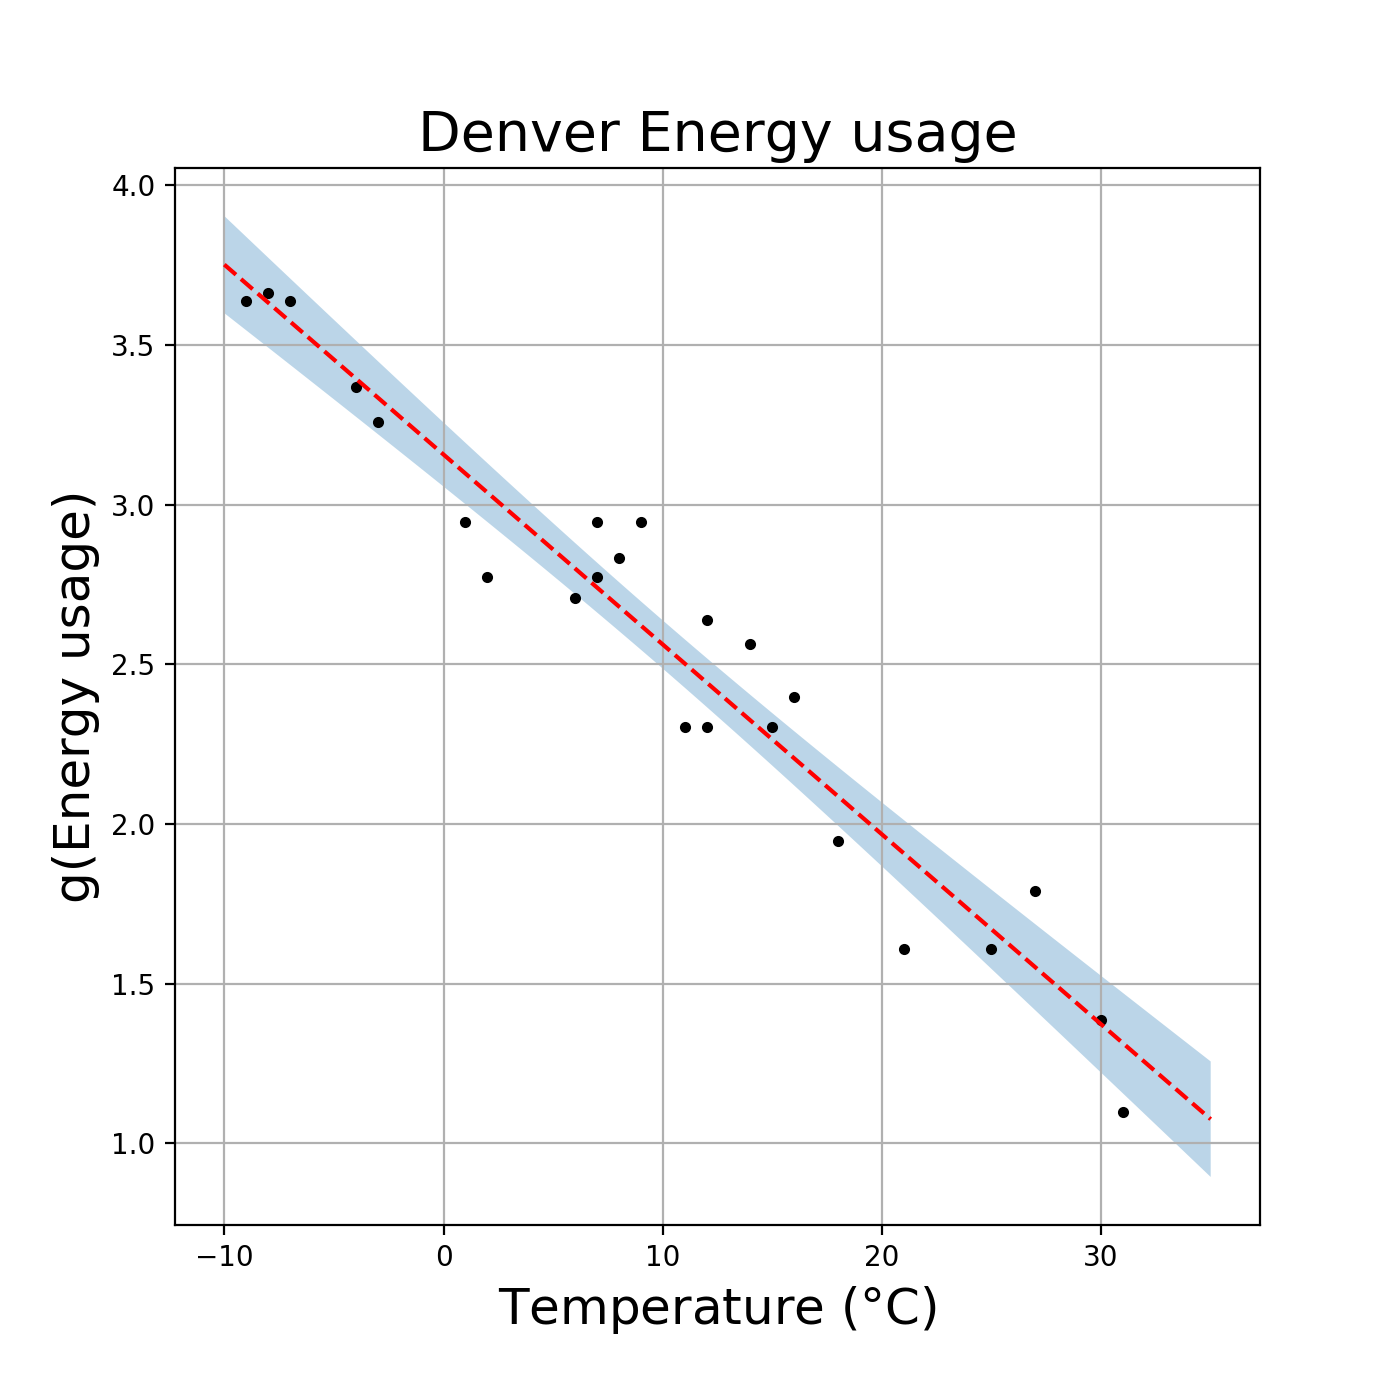
\includegraphics[width=\textwidth]{denver_fit.png}
    \caption{Linear regression fit and confidence intervals for the transformed energy usage vs temperature data for Denver, CO only.}
    \label{fig:denver_fit}
  \end{subfigure}%
  \hfill
  \begin{subfigure}{0.32\textwidth}
    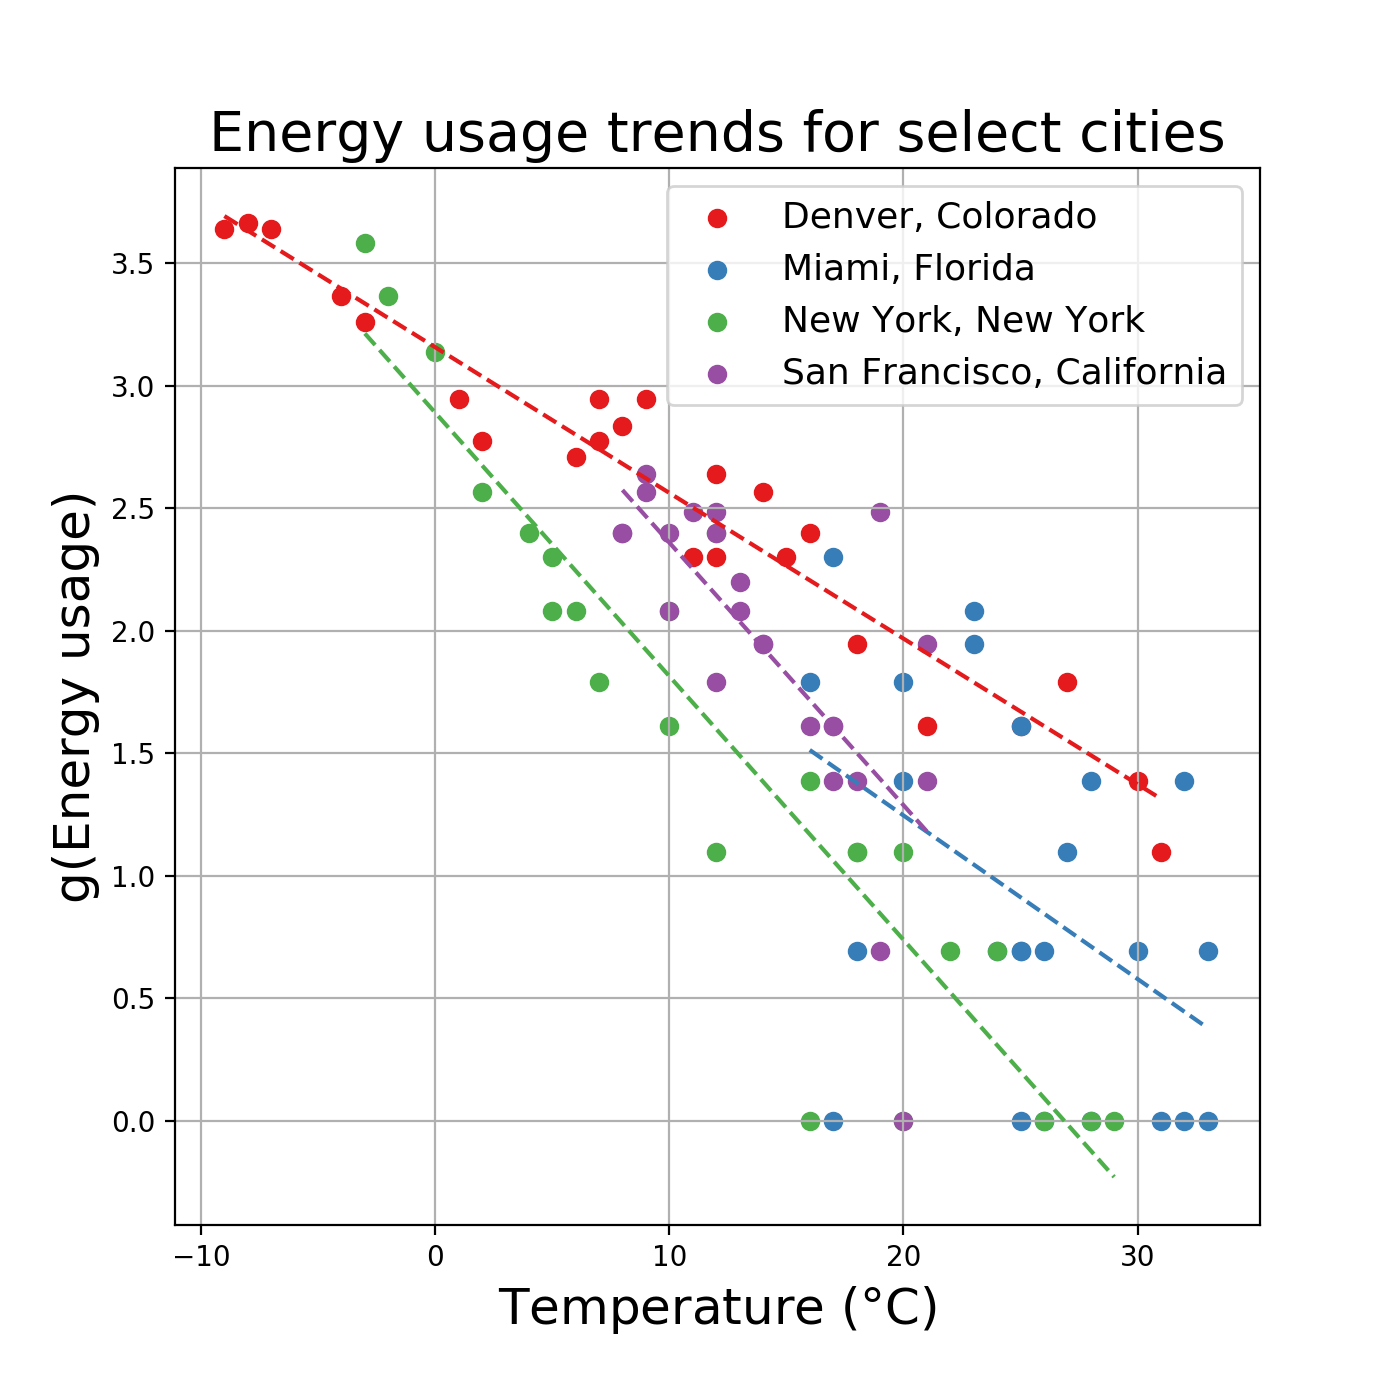
\includegraphics[width=\textwidth]{select_cities.png}
    \caption{Linear regression fits for the transformed energy usage vs temperature data for select cities independent from other cities' data.}
    \label{fig:select_cities}
  \end{subfigure}
  \begin{subfigure}{0.32\textwidth}
    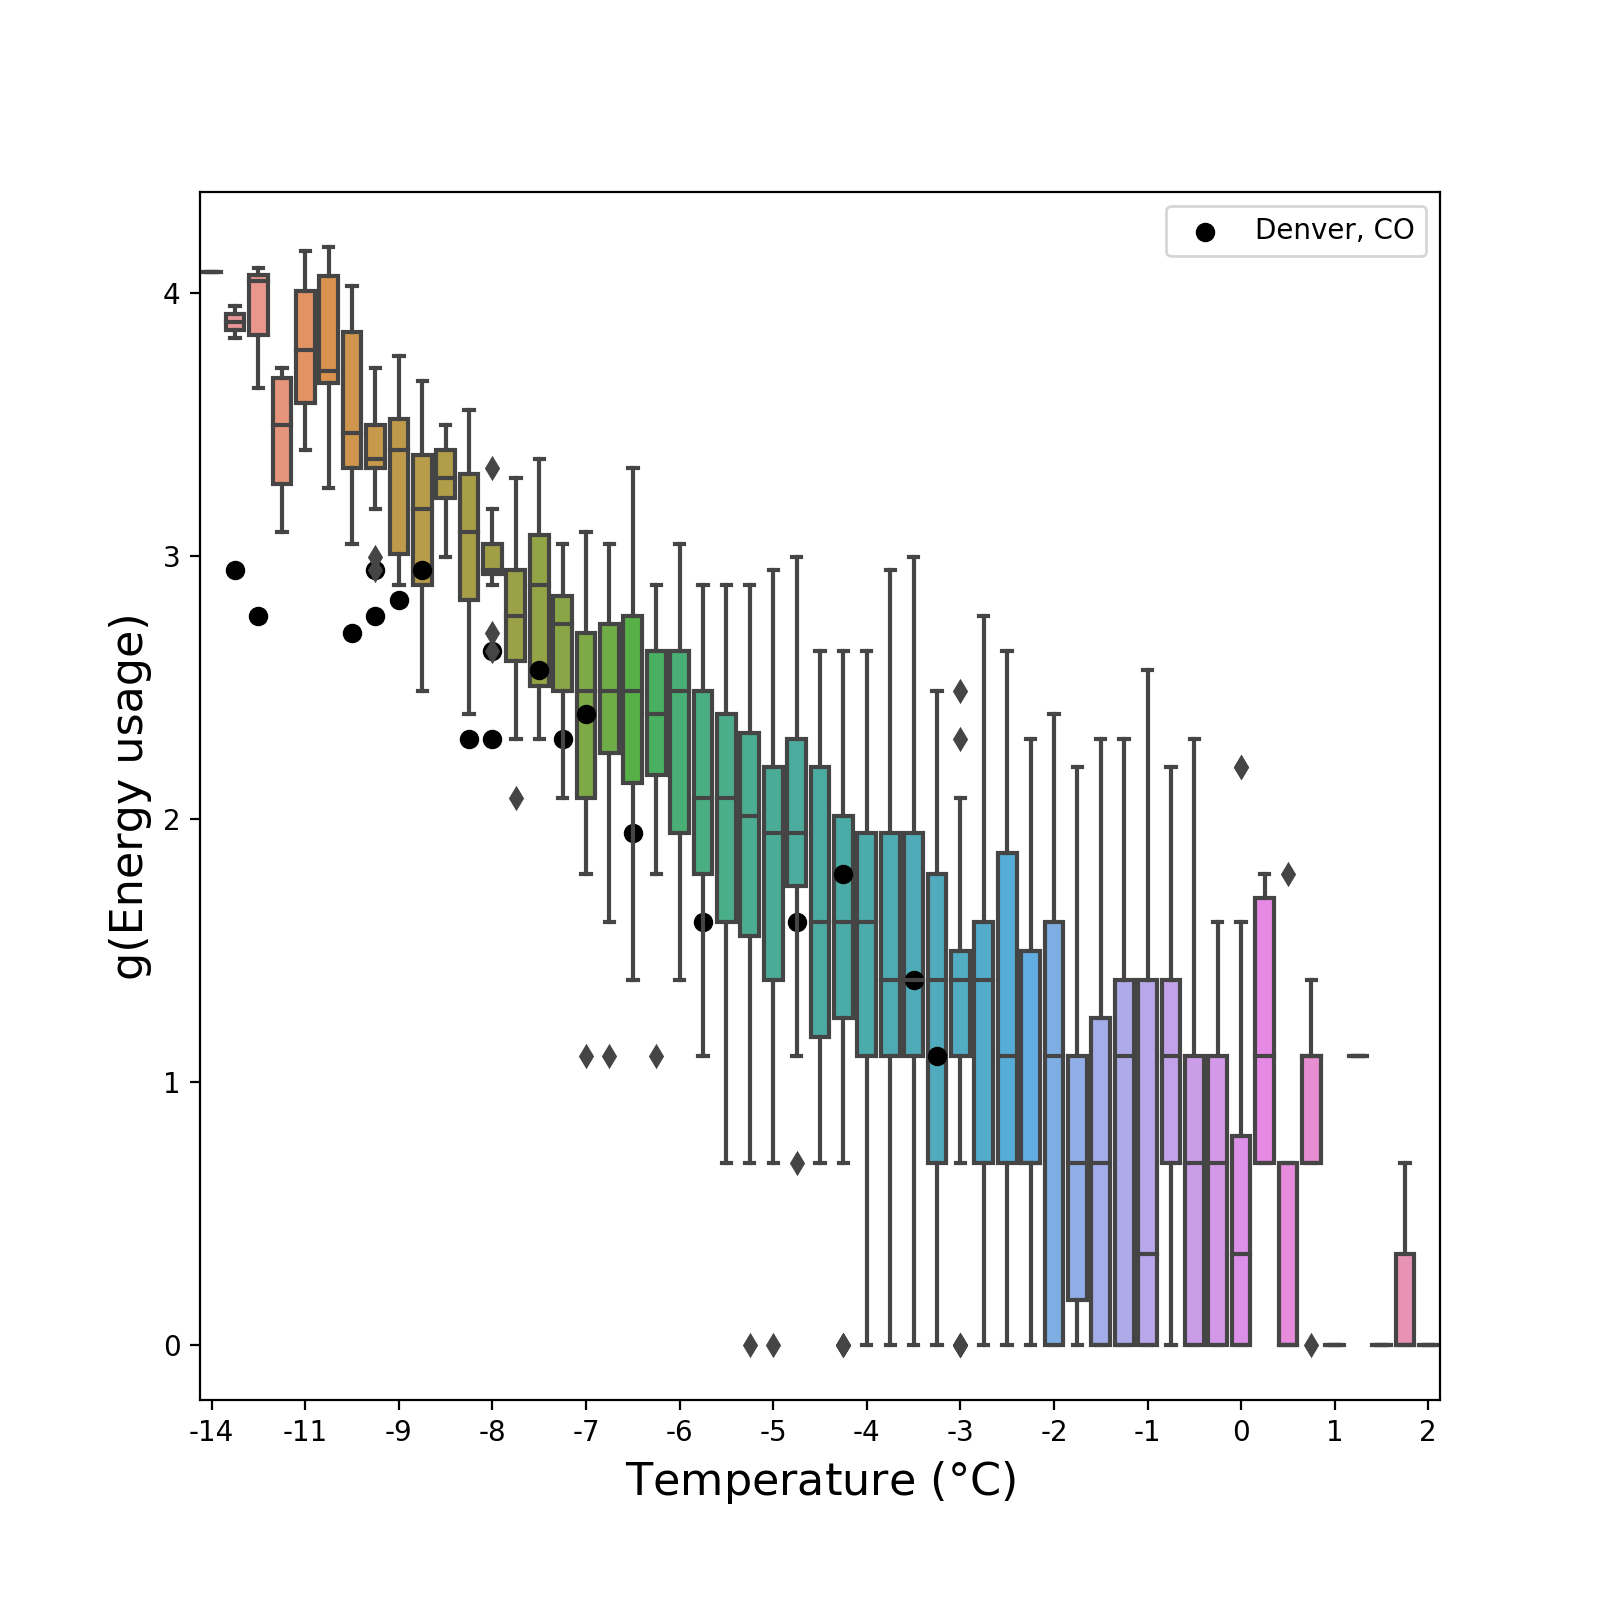
\includegraphics[width=\textwidth]{denver_relative_pooled.png}
    \caption{A box plot summarizing the behavior of the overall population of different cities when comparing transformed energy usage and temperature. Observations of Denver stand out as outliers relative to the behavior of the population, indicating a pooled model would not be appropriate.}
    \label{fig:relative_pooled}
  \end{subfigure}%
  \caption{Linear regression performed using transformed data for single cities. Figures b) and c) also highlight the differences between cities, which motivates using a hierarchical model with city-dependent random effects.}
\end{figure}

\section{\label{sec:model}Model Selection}
 
Since the goal of the model is to predict data for Denver, Colorado, I begin by first examining how a simple linear regression performs on the log-transformed energy vs temperature data. Fig.~\ref{fig:denver_fit} demonstrates the strength of this transformation. Qualitatively, the transformed data linearizes the Denver data very nicely, and a linear regression for Denver alone results in a $R^2$ value of $0.94$. In addition, the residuals plotted vs fitted values (Fig.~\ref{fig:denver_resid}) is nicely distributed, suggesting that the assumption of linearity is valid. Furthermore, a Q-Q plot (Fig.~\ref{fig:denver_qq}) comparing the theoretical quantiles tells us that the assumption of normality is also upheld. Lastly, a leverage plot (Fig.~\ref{fig:denver_leverage}) shows that there are no observations for the city of Denver that are leverage points. All this builds a reasonable case that a very simple model that only considers observations from Denver should be considered.

\begin{figure}[ht] \centering
  \begin{subfigure}{0.32\textwidth}
    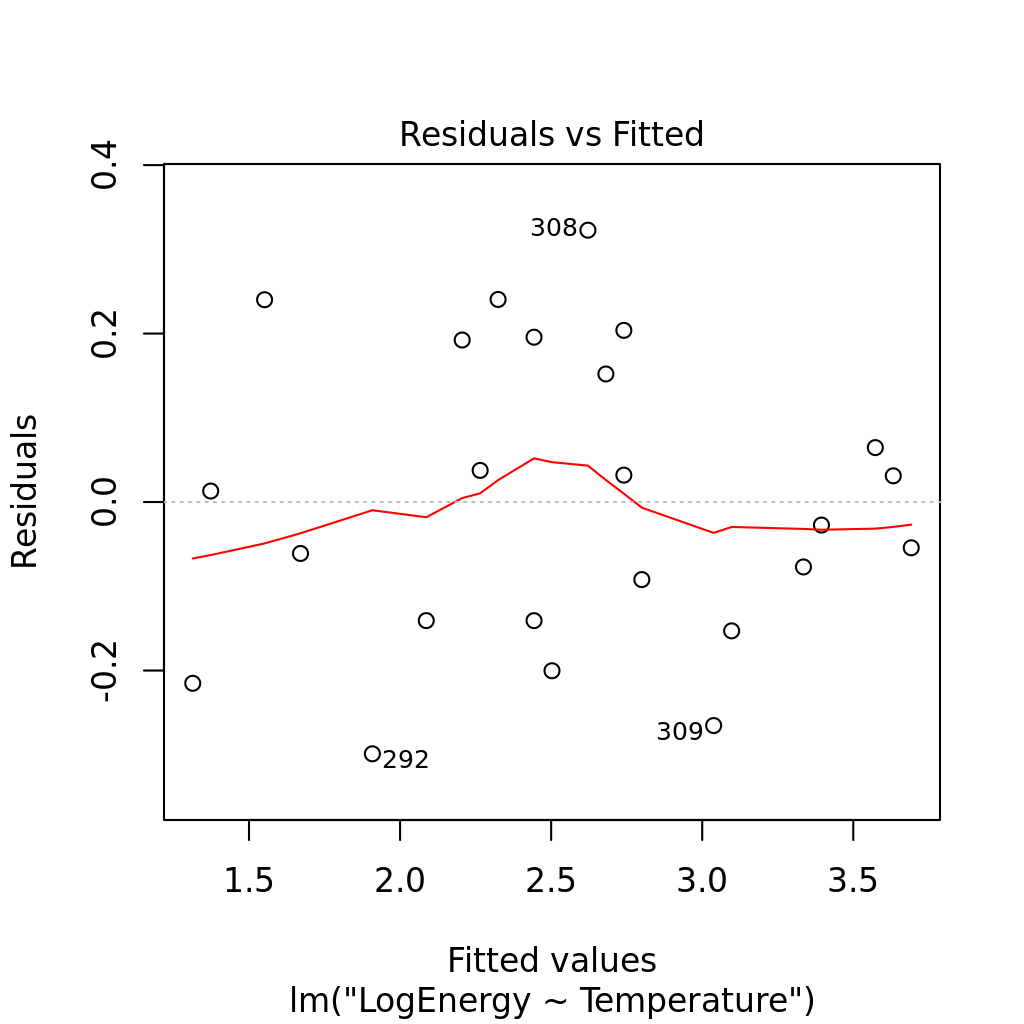
\includegraphics[width=\textwidth]{denver_diagnostic001.png}
    \caption{Residuals vs fitted values.}
    \label{fig:denver_resid}
  \end{subfigure}%
  \hfill
  \begin{subfigure}{0.32\textwidth}
    
\includegraphics[width=\textwidth]{denver_diagnostic002.png}
    \caption{Normal Q-Q plot.}
    \label{fig:denver_qq}
  \end{subfigure}%
  \hfill
  \begin{subfigure}{0.32\textwidth}
    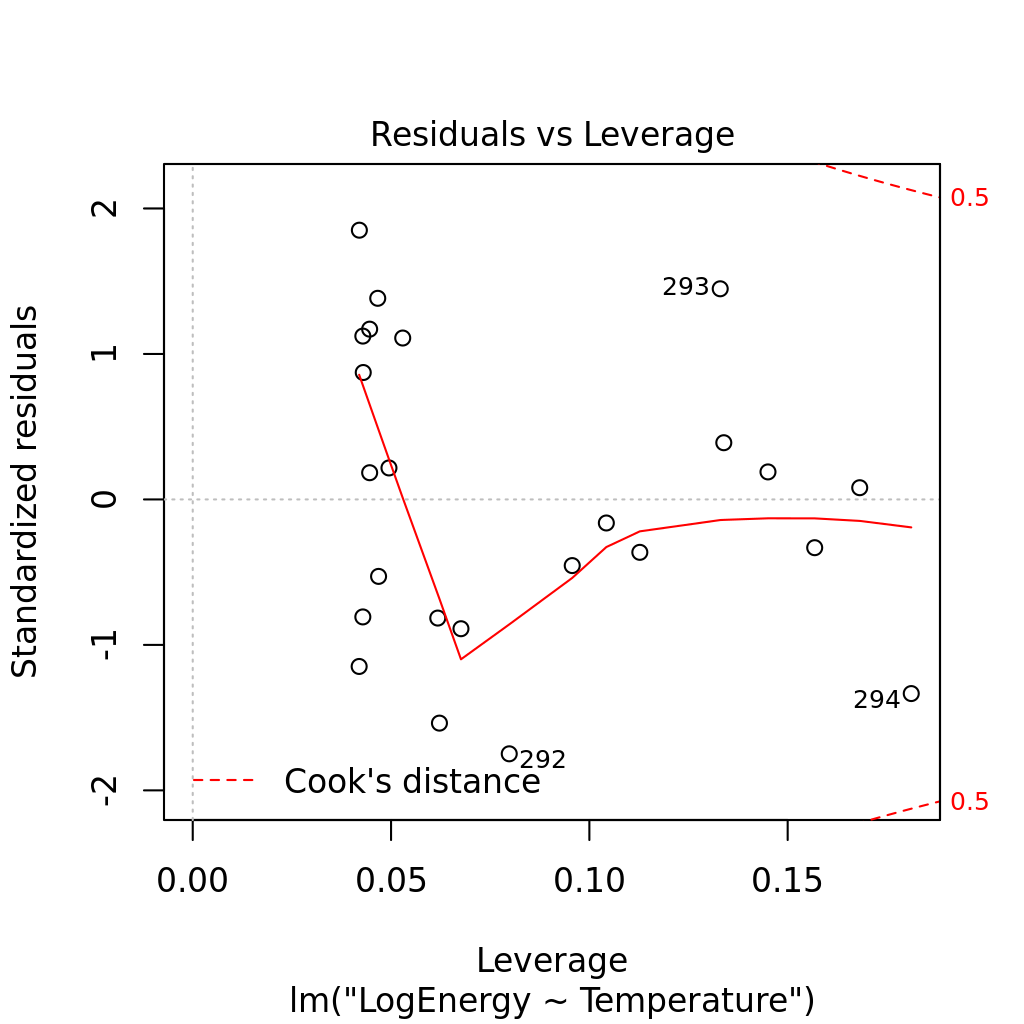
\includegraphics[width=\textwidth]{denver_diagnostic004.png}
    \caption{Leverage plot.}
    \label{fig:denver_leverage}
  \end{subfigure}%
  \caption{Diagnostics of linear-regression fit for transformed energy usage vs temperature for the city of Denver, CO only.}
\end{figure}

Given that the overall trend of the energy/temperature relationship is preserved across different cities (as seen in the exploratory analysis) it would be helpful to use that data to capture the underlying structure (as well as variability) into our model. To verify that the transformation in Eqn.~\ref{eqn:g} is suitable for the aggregated city data, I repeated the diagnostics described above for the pooled city model, and found no signs of linearity or normality violations, nor considerable leverage points. However, as can be see in Fig.~\ref{fig:select_cities}, the data for different cities does not exhibit identical behavior as that seen in the trend for Denver. In fact, comparing the trend for Denver to a pooled model in a box plot (Fig.~\ref{fig:relative_pooled}), the Denver observations appear to be outliers relative to the average trend of the aggregated data. It's therefore clear that a pooled model would not provide an accurate prediction for the city of Denver.


However, it would not do to simply discard the information provided by other cities. Instead, it would be best to incorporate all the data into a hierarchical model. Given that both the temperature dependence and intercept of the data depends strongly on city, it would good to use a mixed effects model with city-dependent random effects for both temperature and intercept. This way we can use the data of all cities to inform how variable we might expect future data to be, while our predictions will best fit the trend that Denver has seen historically. Our model in this case will be
\begin{equation} \label{eqn:mod}
  g(E_{jk}+1) = \beta_0 + a_j + (\beta_1 + b_j)T_k + e_{jk},
\end{equation}
where $E_{jk}$ is the energy usage (in hundreds of GWh) for city $j$ at time $k$, $T_{jk}$ is the temperature (in $^\circ$C) in city $j$ at time $k$, $\beta_0$ and $\beta_1$ are the fixed intercept and slope for the population of cities, $a_j$ and $b_j$ are the differences of these parameters for the specific city $j$, and $e_jk$ is a noise term. This model incorporates the best of both worlds---a mix between a simple, yet well-fit model that only considers Denver's data for the purpose of predicting more data from Denver, and a model that incorporates all the data available from 50 other cities in the US.
%\begin{figure}[ht] \centering
  %\hfill
  %\begin{subfigure}{0.49\textwidth}
    %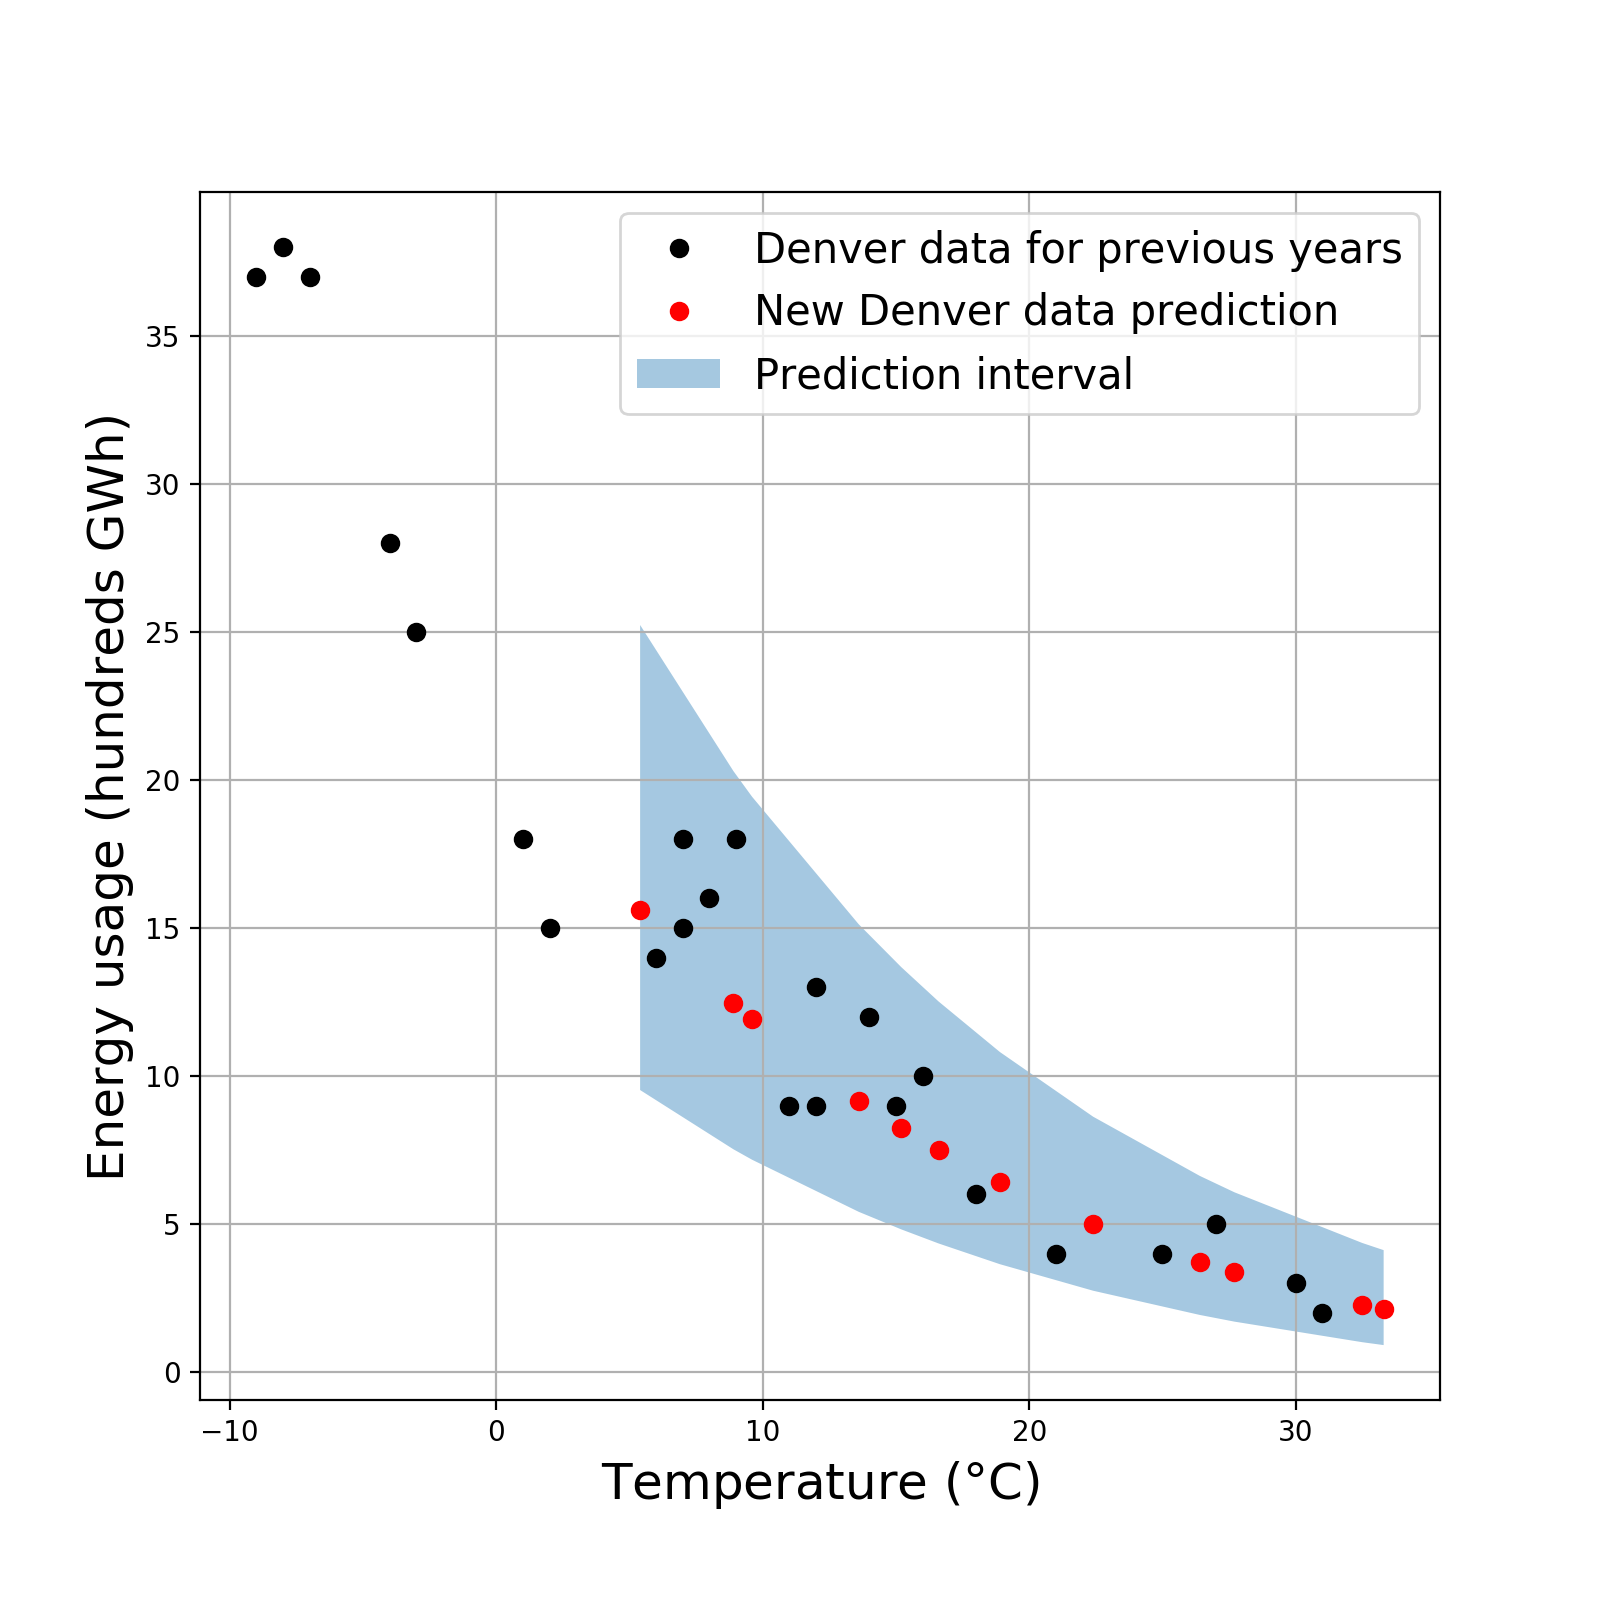
\includegraphics[width=\textwidth]{denver_predictions.png}
    %\caption{Predictions and 95\% prediction intervals for third year of data from Denver, CO. To compare, I have also plotted the known Denver data from previous years. Prediction intervals were calculated from both fixed effects uncertainty plus the random effects variance by computing $XVX^T$ (where $X$ is the matrix of the new Denver data, and $V$ is the variance-covariance matrix from parameters $\boldsymbol{\beta}$), as well as adding the residual variance (note that this is the method outlined by Ben Bolker at http://bbolker.github.io/mixedmodels-misc/glmmFAQ.html).}
    %\label{fig:prediction}
  %\end{subfigure}
%\end{figure}

\section{\label{sec:results}Model Results and Analyses}

In order to fit the model described by Eqn.~\ref{eqn:mod}, I used the $lmer$ function in R's $lme4$ package, including random effects for both intercept and temperature by city. The function finds the fixed effect values of $\beta_0 = 2.94 \pm 0.04, \beta_1 = -0.078 \pm 0.003$, and each are extremely significant with t-value magnitudes $>25$. The standard deviations of the random effects based on city are $0.23$ for the intercept random effects and $0.02$ for temperature.

For a goodness-of-fit criterion, I calculate $\Omega_0^2$ (a kind of pseudo-$R^2$) of the model by comparing the variance of the full model with the variance of a fixed, intercept-only model $\Omega_0^2 = 1-Var(M_{full})/Var(M_{null})$. For this model, I find $\Omega_0^2 = 0.84$. Given the high variance in the data, I believe this model explains an acceptable fraction. In addition, the residuals vs fitted values are well-distributed without any sign of violations of linearity.

The model parameters $\boldsymbol{\beta}$ as well as the random effects for the city of Denver, CO were used to make predictions given the temperature data from Denver for the third year. These predictions, as well as calculated prediction intervals, are shown in Fig.~\ref{fig:prediction}. Included in the figure are the Denver observations from previous years. As a sanity check, it is good to see that all the previous observations fall into the range of the prediction interval, and the predictions for the new temperature data seem reasonable qualitatively. 

In order to determine whether the random effects are significant, I fitted two reduced models: one model with no random effects and one model with only intercept random effects based on city. I then performed a likelihood ratio test using R's $anova$ function, and found that the full model with random effects for both intercept and temperature was extremely significant ($p<2.2\times10^{-16}$), justifying the use of random effects for both intercept and temperature.

\begin{figure}[ht] \centering
  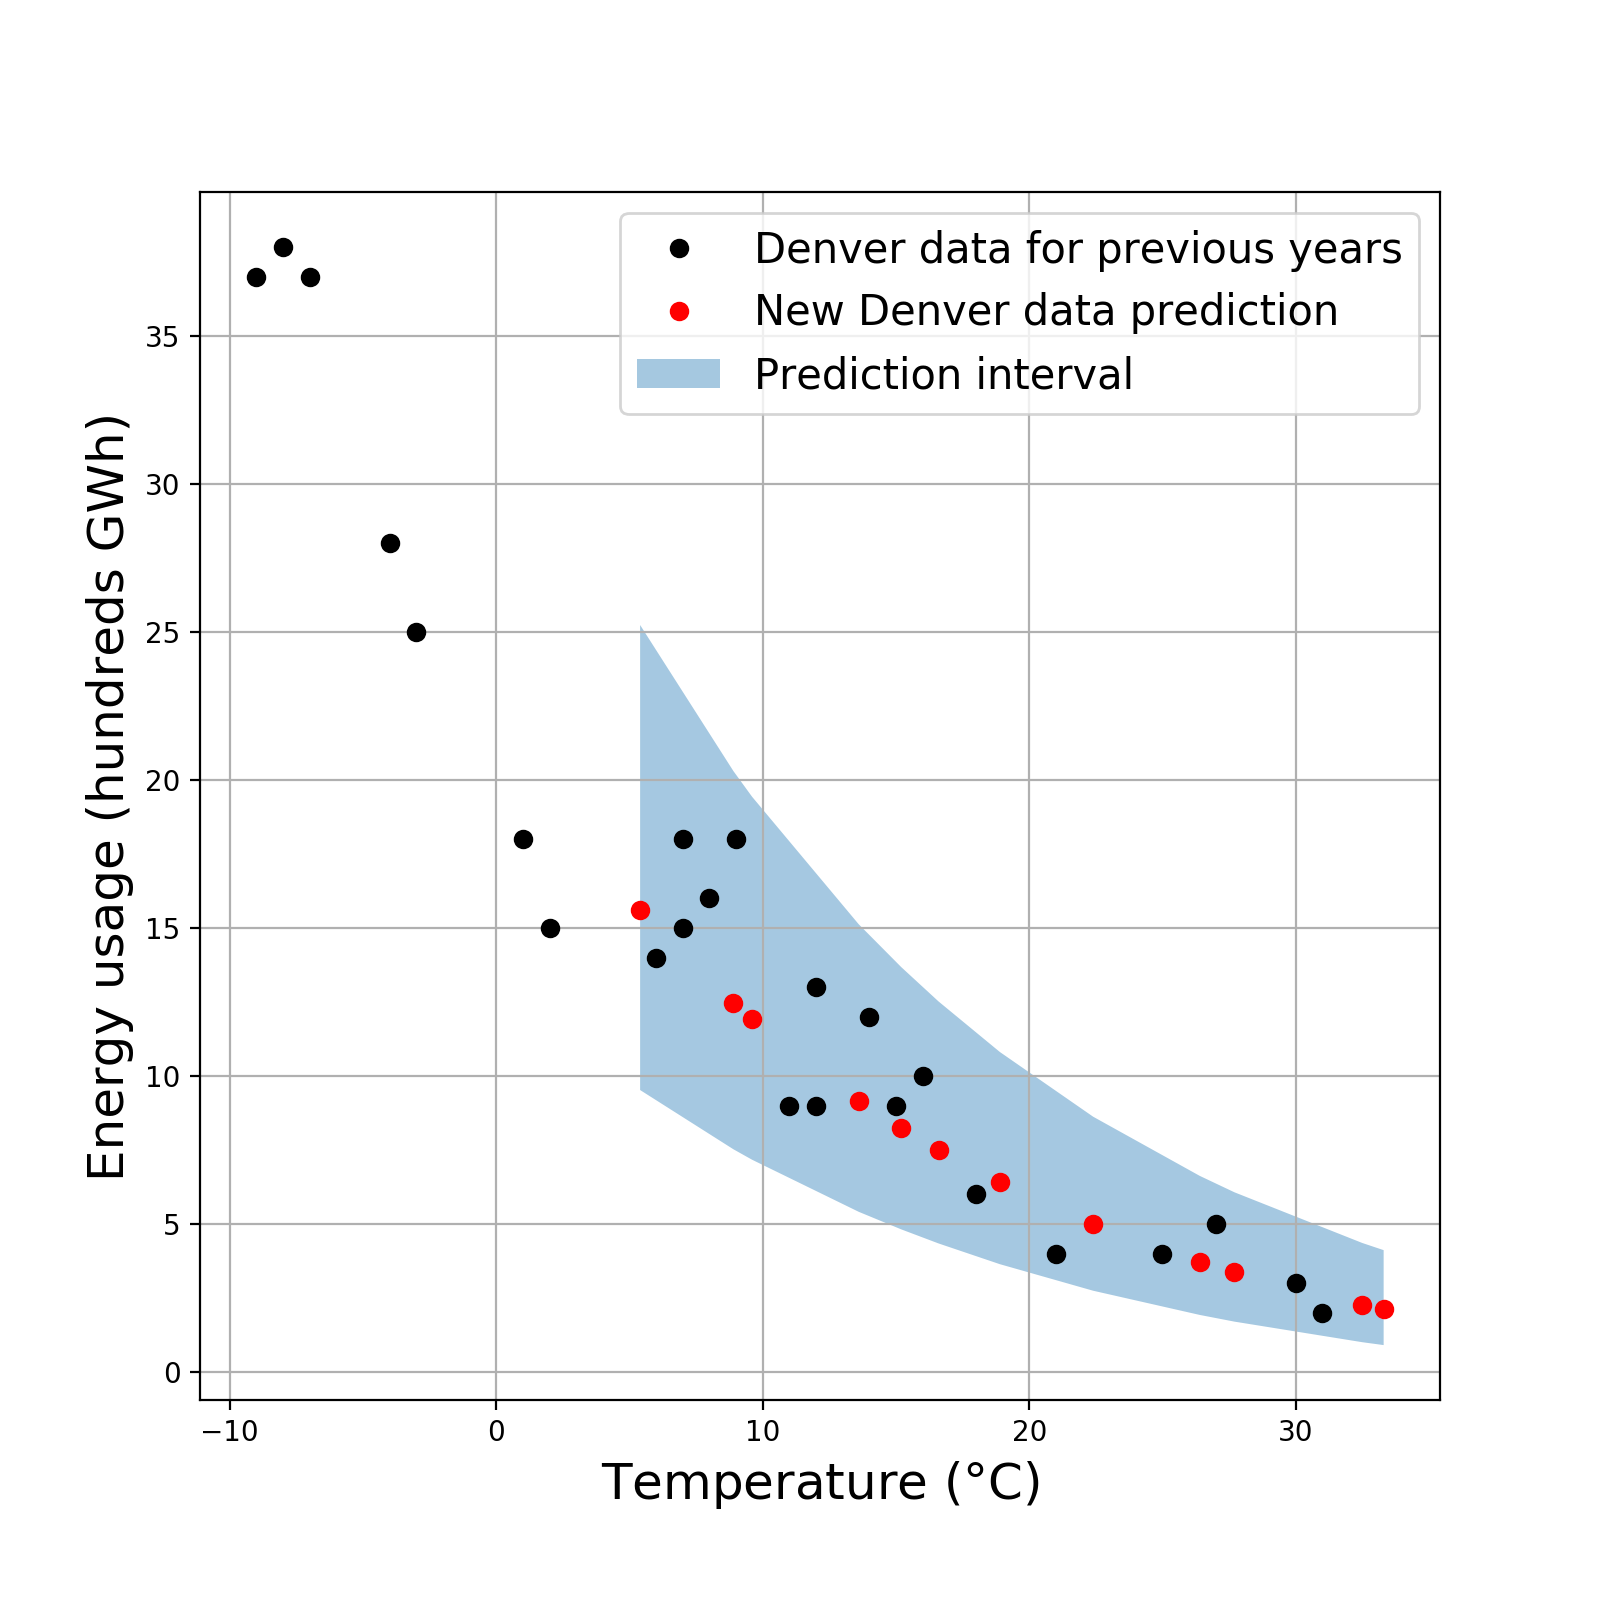
\includegraphics[width=0.65\textwidth]{denver_predictions.png}
  \caption{Predictions and 95\% prediction intervals for third year of data from Denver, CO. To compare, I have also plotted the known Denver data from previous years. Prediction intervals were calculated from both fixed effects uncertainty plus the random effects variance by computing $XVX^T$ (where $X$ is the matrix of the new Denver data, and $V$ is the variance-covariance matrix from parameters $\boldsymbol{\beta}$), as well as adding the residual variance (note that this is the method outlined by Ben Bolker at http://bbolker.github.io/mixedmodels-misc/glmmFAQ.html).}
  \label{fig:prediction}
\end{figure}

\section{\label{sec:conclusion}Conclusions and Future Extensions}

There are several alternative approaches to the model I described above that could be worth considering, at the risk of adding more complexity to the model. Here I will list a couple alternative approaches that I would explore in order to further optimize my model selection.

First, I could use a Box-Cox transformation to tune my transformation function more finely, rather than the simple logarithmic transformation described by Eqn.~\ref{eqn:g}. This would test my assumption that the energy usage increases exponentially with colder temperatures. I could then compare the performance of a mixed random effects model using both of these approaches by comparing the model likelihoods.

Next, I could attempt to fit a generalized linear mixed effect model using the Poisson family and compare that to my current approach. Since there appears to be an increase in the variance of the data with increasing temperatures, this would be a natural model to compare to my current model.

Finally, I have not attempted to quantify any potential zero-inflation in my data. Future approaches could do this by using more specialized R packages that could account for zero-inflation and compare its performance and likelihood to models without this consideration.

Given the significance of the random effects for the mixed effects model, goodness-of-fit (respectable $\Omega_0^2$), qualitative performance of the calculated prediction interval compared to historical data, I believe the model described above is a good balance between simplicity and complexity. I am reasonably confident in the accuracy of its performance and simultaneously curious to see how my predictions would measure up to the truth.

%\begin{algorithm}
  %\DontPrintSemicolon
  %Models: \\
%m0: LogEnergy $\sim$ Temperature \\
%m1: LogEnergy $\sim$ Temperature + (1 $\vert$ City) \\
%m2: LogEnergy $\sim$ Temperature + (1 $\vert$ City) + (0 + Temperature $\vert$ City) \\
   %Df    AIC    BIC   logLik deviance  Chisq Chi Df Pr(>Chisq) \\
%m0  3 2214.5 2229.8 -1104.25   2208.5 \\
%m1  4 1751.8 1772.3  -871.92   1743.8 464.65      1  < 2.2e-16 *** \\
%m2  5 1577.1 1602.7  -783.55   1567.1 176.75      1  < 2.2e-16 *** \\
  %\caption{anova output for R}
%\end{algorithm}

%%%%%%%%%%%%%%%%%%%%%%%%%%%%%%%%%%%%%%%%

%%% Use for standard bibliography %%%
%\bibliographystyle{unsrt} \bibliography{bib-file-name}

%%% Use for REVTEX4 bibliography %%% 
%\bibliography{bib-file-name}

\end{document}
